\chapterimage{chapter_head_1.png}

\chapter{Suchalgorithmen für Spiele}

\usetikzlibrary{arrows}
\usetikzlibrary{calc}
\usetikzlibrary{positioning}
\usetikzlibrary{matrix}

\pgfdeclarelayer{background}
\pgfsetlayers{background,main}

\tikzset{
    treenode/.style = {align=center, inner sep=0pt, text centered,
        font=\sffamily},
    arn_n/.style = {treenode, circle, white, font=\sffamily\bfseries, draw=blue, fill=blue,
        text width=1.5em, minimum width=1.5em, minimum height=1.5em},% arbre rouge noir, noeud noir
    arn_r/.style = {treenode, circle, white, draw=red, fill=red, 
        text width=1.5em, very thick, minimum width=1.5em, minimum height=1.5em},% arbre rouge noir, noeud rouge
    arn_x/.style = {treenode, rectangle, draw=black,
        minimum width=1.5em, minimum height=1.5em},% arbre rouge noir, nil
}


\section{Intro \& Motivation}

In den vorangegangenen Kapiteln haben wir schon einige Suchverfahren kennengelernt, welche uns nun helfen werden Algorithmen zu verstehen, die verwendet werden um Computergegner für Nullsummenspiele zu entwickeln. Hierbei werden wir uns den Minimax-Algorithmus, sowie den Alpha-Beta-Algorithmus genauer anschauen, welche beide versuchen sich in die Lage des Gegners zu versetzen, um so  herauszufinden, welche Reaktion dieser auf einen Zug von uns wählen würde. Ziel der Algorithmen ist es, ein für uns bestmögliches Ergebnis und somit, wenn möglich, einen Sieg zu erlangen. Dieses Vorgehen kann eine Betrachtung von sehr vielen möglichen Züge zur Folge haben, was sehr viel Rechenaufwand bedeutet. Im Folgenden werden wir jedoch  mit Hilfe des Alpha-Beta-Algorithmus eine Methode kennenlernen, die es uns ermöglicht die Anzahl der zu betrachtenden Züge zu reduzieren.



\section{Inhaltliche Ausarbeitung des Themas}

Wir betrachten ein Nullsummenspiel, was bedeutet, dass der Gewinn des einen Spielers (Nutzwert positiv) mit dem Verlust des Gegners (Nutzwert negativ) äquivalent ist und ein Unentschieden keine Auswirkungen auf die Nullsummeneigenschaft hat (Nutzwert 0).
Gegeben sei für dieses Spiel ein Spielbaum $T = (V;E)$. Bei einem gleichförmigen Spielbaum besitzt jeder innere Knoten den gleichen Verzweigungsgrad b und alle Blätter befinden sich in der gleichen Tiefe d, sodass die Zahl der Knoten in einem gleichförmigen Baum exponentiell mit der Tiefe des Baumes wächst ($b^d$). Jedoch gibt es auch Spielbäume bei denen der Verzweigungsgrad der Ebenen variiert.
Der Spielbaum beinhaltet alle möglichen Züge und Spielausgänge. Die Tiefe und der Verzweigungsgrad hängt von dem Spiel ab, welches wir betrachten. Beispielsweise hat der Spielbaum zu einem Tic-Tac-Toe Spiel eine Tiefe von 9 (da es 9 Felder zu besetzen gibt) und zu Beginn des Spiels einen Verzweigungsgrad von 9 (weil noch alle 9 Felder zur Auswahl stehen), der mit wachsender Tiefe allerdings abnimmt, da nach jedem Zug immer ein leeres Feld weniger vorhanden ist.



\subsection{Problemstellung}
Zu dem gegebenen Nullsummenspiel wollen wir einen Computergegner programmieren, der in der Lage ist die optimale Antwort auf jede Spielposition, bei optimalem Spiel beider Spieler, zu finden.
Dafür müssen wir jedoch vorher festlegen, was für uns optimal in diesem Zusammenhang bedeutet. Wir gehen davon aus, dass der Gegner immer den für ihn optimalen Zug wählt, d.~h. den Zug, der für ihn zum besten Nutzwert und somit für uns zum schlechtesten Nutzwert führt. Analog wollen wir agieren. Wie dies genau funktioniert werden wir im folgenden Abschnitt sehen.



\subsection{Methoden}


\subsubsection*{Minimax Algorithmus}
Im folgenden bezeichnen wir unseren Spieler mit MAX und den gegnerischen Spieler mit MIN. Wie zuvor schon angedeutet ist das Ziel des Minimax-Algorithmus den Minimax-Wert für die aktuelle Stellung zu bestimmen. Der Minimax-Wert der Endstellungen (Blätter) entspricht dem Nutzwert für MAX. Die Berechnung der anderen Knoten erfolgt rekursiv mit Hilfe der folgenden Bewertungsfunktion:

\begin{center}
	$Minimax(k) = \begin{cases} Nutzwert(k) & \mathrm{falls}~k~\mathrm{Endzustand}\\
		max\{minimax(t) ~|~ t \in N(t)\} 	& \mathrm{falls}~k~\mathrm{MAX\hbox{-}Knoten}\\
		min\{minimax(t) ~|~ t \in N(t)\}	& \mathrm{falls}~k~\mathrm{MIN\hbox{-}Knoten}	\end{cases} $
\end{center}

wobei $N(t)$ die Funktion ist, die die Kinder im Baum liefert. Die Auswertung der Knoten geschieht Bottom up, das bedeutet wir beginnen bei den Blättern und bewerten von dort ausgehend die Elternknoten und anschließend deren Eltern bis wir irgendwann bei der Wurzel angelangt sind. Der Minimax Algorithmus liefert nicht unbedingt den höchsten Nutzwert der Blätter, sondern den größten Nutzwert den man erhalten kann, wenn der Gegner selbst versucht zu gewinnen und somit den Nutzwert für uns möglichst klein zu halten.\\

Anschaulicher wird das ganze, wenn man sich den Algorithmus an einem Beispiel anschaut.

\textbf{Beispiel}\\

Gegeben sei der folgende Spielbaum
\begin{center}
\includegraphics[width = 7 cm]{chapters/minimax/jpg/Graph-Minmax1.jpg}
\end{center}

Angenommen MIN wäre an der markierten Position:
\begin{center}
	\includegraphics[width = 7 cm]{chapters/minimax/jpg/Graph-Minmax2-1.jpg}
\end{center}

Dann würde MIN den Zug auswählen, der für ihn den größten Nutzwert und somit für uns den kleinsten Nutzwert hat. Das heißt in dem Fall:
\begin{center}
	 $min\{minimax(t) | t \in N(t)\} ~=~ min\{9,3\} ~=~ 3$

\includegraphics[width = 7 cm]{chapters/minimax/jpg/Graph-Minmax2-2.jpg}
\end{center}

Angenommen MIN wäre an der markierten Position:
\begin{center}
	\includegraphics[width = 7 cm]{chapters/minimax/jpg/Graph-Minmax2-3.jpg}
\end{center}

Dann würde MIN den Zug auswählen, der für ihn den größten Nutzwert und somit für uns den kleinsten Nutzwert hat. Das heißt in dem Fall:
\begin{center}
	$min\{minimax(t) | t \in N(t)\} ~=~ min\{1,5\} ~=~ 1$

	\includegraphics[width = 7 cm]{chapters/minimax/jpg/Graph-Minmax2-4.jpg}
\end{center}

Nun betrachten wir den Zug von MAX. Der Suchbaum sieht wie folgt aus

\begin{center}
	\includegraphics[width = 7 cm]{chapters/minimax/jpg/Graph-Minmax2.jpg}
\end{center}

MAX würde den Zug wählen, der für ihn den höchsten Nutzwert hat.\\

\begin{center}
	$max\{minimax(t) | t \in N(t)\} ~=~ max\{3,1\} ~=~ 3$
	\includegraphics[width = 7 cm]{chapters/minimax/jpg/Graph-Minmax3.jpg}
\end{center}

Somit sieht der Suchbaum nach Abschluss des Minimax-Algorithmus wie folgt aus, wobei der rote Pfad den optimalen Nutzwert liefert, wenn beide Spieler optimal spielen. Somit sollte MAX den linken Knoten wählen.

\begin{center}
	\includegraphics[width = 7 cm]{chapters/minimax/jpg/Graph-Minmax4.jpg}
\end{center}

\vskip 60pt



\subsubsection*{Problem:} Der Minimax-Algorithmus durchsucht den Suchbaum $T=(V, E)$ mit Tiefensuche, in der Zeit $O(max \{|V|, |E|\}) = O(|V|)$. Somit benötigt die Suche zwar lineare Zeit, jedoch wächst der Baum exponentiell mit zunehmender Tiefe ($O(|V|)=O(b^d)$). Somit ist der Algorithmus für Bäume mit großer Tiefe ineffizient.


\subsubsection*{Alpha-Beta-Algorithmus}
 Der Alpha-Beta-Algorithmus ist eine Verbesserung vom Minimax-Algorithmus, da die Zugriffsanzahl reduziert wird, indem Teile des Suchbaums nicht durchsucht werden, ohne dabei das Ergebnis zu verfälschen. Für die Umsetzung werden die Variablen $\alpha$ und $\beta$ eingeführt, wobei $\alpha$ der Nutzwert ist, welchen MAX mindestens erreicht und $\beta$ der Nutzwert, den MIN höchstens erreicht. Die Auswertung der Knoten geschieht on-the-fly, d.~h. nur dann, wenn wir sie wirklich benötigen. \\

 \underline{MAX-Knoten:}\\
 Betrachten wir einen MAX Knoten und stellen dort einen Wert fest, der größer ist als $\beta$, brauchen wir den Teilbaum nicht weiter betrachten, da MIN diesen nicht wählen würde, weil der andere Teilbaum einen kleineren Nutzwert liefert. Das nicht weiter Betrachten des Teilbaums bezeichnet man als Beta-Cutoff. Ist  der Wert des MAX Knoten größer als $\alpha$ erhöht sich der Wert den MAX mindestens erreicht und wir aktualisieren $\alpha$ auf den Wert des Knotens.  \\

 \underline{MIN-Knoten:}\\
 Ist der Wert eines MIN Knotens kleiner als der Wert von $\alpha$ müssen wir diesen Teilbaum nicht weiter analysieren, da MAX immer den Teilbaum mit dem größten Nutzwert auswählt und da $\alpha$ größer ist als der Wert des betrachteten Knotens existiert ein Teilbaum mit einem größeren Nutzwert. Also würde hier ein Cutoff stattfinden, welchen man als Alpha-Cutoff bezeichnet. Sollte jedoch der Wert des MIN Knotens größer als $\beta$ sein steigt der Wert den MIN höchstens erreicht und wir müssen $\beta$ auf diesen Wert anpassen.


 \begin{algorithm}
 	\KwData{Graph $G=(V,E)$, Blätter mit Nutzwert, s = Knoten}
 	\KwResult{Nutzwert für jeden knoten}
 	\textbf{alpha-beta-suche(s)}\\

 	\textbf{return} maximalerWert(s, -$\infty$, $\infty$)\\

 	\textbf{maximalerWert}(Knoten, $\alpha$, $\beta$)\\

	 	\If{s = Blatt}{
	 		\textbf{return} wert(s)
	 	}
	 	\Else{
	 		$wert = \alpha$\\
	 		\ForEach{k= Kind(s)}{
		 		$wert = max\{wert, minimalerWert(k, wert, \beta)\}$\\
		 		\If {$wert >= \beta$}{
			 		\textbf{return} wert}
			 	$\alpha = max\{\alpha, wert\}$\\
	 		}
			\textbf{return} wert
	 	}

	\textbf{minimalerWert}(Knoten, $\alpha$, $\beta$)\\

	\If{s = Blatt}{
		\textbf{return} wert(s)
	}
	\Else{
		$wert = \beta$\\
		\ForEach{k= Kind(Knoten)}{
			$wert = min\{wert, minimalerWert(k, \alpha, wert)\}$\\
			\If {$wert <= \alpha$}{
				\textbf{return} wert}
			$\beta = min\{\beta, wert\}$\\
		}
		\textbf{return} wert

	}
 	\caption{Alpha-Beta-Algorithmus}
\end{algorithm}

Betrachten wir ein Beispiel, um den Algorithmus besser zu verstehen.

\paragraph{Beispiel:}

Gegeben sei der folgender Spielbaum, blaue Knoten sind MAX- und rote MIN-Entscheidungen.
Wir folgen immer den linken Kindern. Zunächst treffen wir unsere erste Entscheidung, dafür müssen beide Kinder des linkesten Pfades evaluiert werden.
Wir entscheiden uns für die 5. Dieser Wert ist der neue $\beta$ -Wert für seinen Schwester-Knoten. Heißt unser Gegenspieler MIN wird sich höchstens für den Wert 5 entscheiden.

\begin{center}
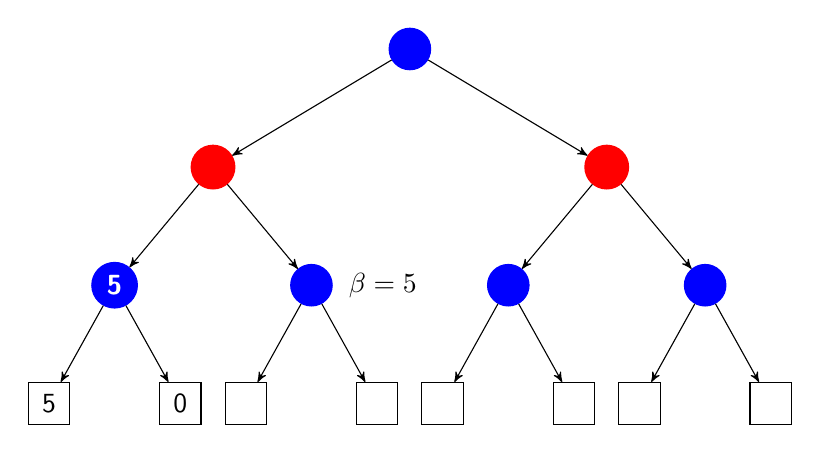
\begin{tikzpicture}[->,>=stealth',level/.style={sibling distance = 5cm/#1,
    level distance = 1.5cm}] 
\node [arn_n] {}
child{ node [arn_r] {} 
    child{ node [arn_n] {5}
        child{ node [arn_x] {5}}
        child{ node [arn_x] {0}} 
    }
    child{ node [arn_n] {}
        child{ node [arn_x] {}}
        child{ node [arn_x] {}}
        node[right = 1em]{$\beta=5$}
    }                            
}
child{ node [arn_r] {}
    child{ node [arn_n] {} 
        child{ node [arn_x] {}}
        child{ node [arn_x] {}}
    }
    child{ node [arn_n] {}
        child{ node [arn_x] {}}
        child{ node [arn_x] {}}
    }
}
; 
\end{tikzpicture}
\end{center}

Wir evaluieren den nächsten Knoten im Nachbar-Graphen. Er ist 6. Da dieser Wert größer-gleich des $\beta$-Wert ist, müssen wir den Rest des Teil-Graphen nicht zu evaluieren. Dies ist überflüßig, da MIN den tiefsten Wert wählen wird, welcher mindestens 5 ist. Wir brauchen also nicht nach einem noch größeren Wert suchen. \\
\textbf{Dies nennt man $\beta-Cut$.} \\
Der neue $\alpha$-Wert des roten Schwester-Konten ist nun 5. Heißt: Wir können danach mindestens eine 5 wählen.

\begin{center}
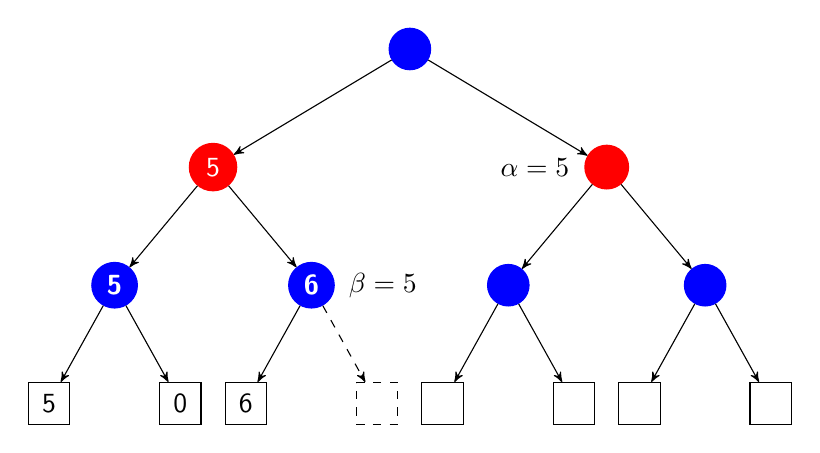
\begin{tikzpicture}[->,>=stealth',level/.style={sibling distance = 5cm/#1,
    level distance = 1.5cm}] 
\node [arn_n] {}
child{ node [arn_r] {5} 
    child{ node [arn_n] {5}
        child{ node [arn_x] {5}}
        child{ node [arn_x] {0}}
    }
    child{ node [arn_n] {6}
        child{ node [arn_x] {6}}
        child[dashed]{ node [arn_x] {}}
        node[right = 1em]{$\beta=5$}
    }                            
}
child{ node [arn_r] {}
    child{ node [arn_n] {} 
        child{ node [arn_x] {}}
        child{ node [arn_x] {}}
    }
    child{ node [arn_n] {}
        child{ node [arn_x] {}}
        child{ node [arn_x] {}}
    }
    node[left = 1em]{$\alpha=5$}
}
; 
\end{tikzpicture}
\end{center}

Da der ganze linke Teilbaum evaluiert ist, kann der rechte Baum evaluiert werden. 
Dort wird wieder dem linkesten Pfad gefolgt. Wir evaluieren und setzen den $\beta$-Wert für den Schwesterknoten genauso wie im linken Teilbaum.

\begin{center}
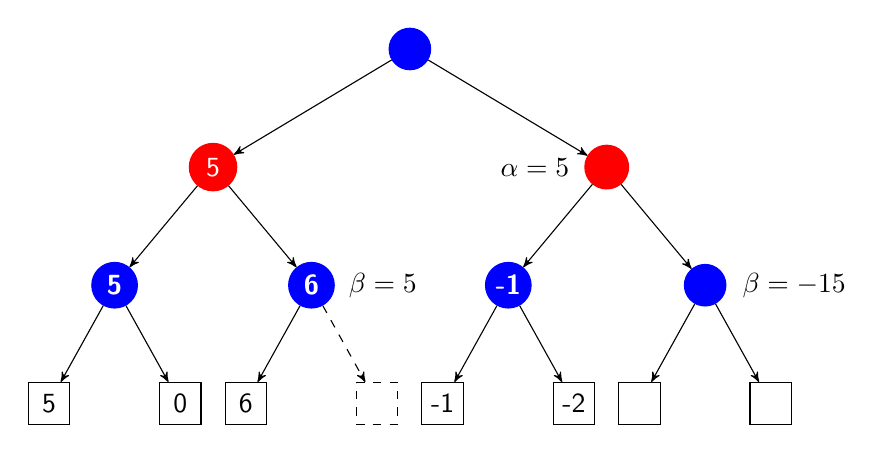
\begin{tikzpicture}[->,>=stealth',level/.style={sibling distance = 5cm/#1,
    level distance = 1.5cm}] 
\node [arn_n] {}
child{ node [arn_r] {5} 
    child{ node [arn_n] {5}
        child{ node [arn_x] {5}}
        child{ node [arn_x] {0}} 
    }
    child{ node [arn_n] {6}
        child{ node [arn_x] {6}}
        child[dashed]{ node [arn_x] {}}
        node[right = 1em]{$\beta=5$}
    }                            
}
child{ node [arn_r] {}
    child{ node [arn_n] {-1} 
        child{ node [arn_x] {-1}}
        child{ node [arn_x] {-2}}
    }
    child{ node [arn_n] {}
        child{ node [arn_x] {}}
        child{ node [arn_x] {}}
        node[right = 1em]{$\beta=-15$}
    }
    node[left = 1em]{$\alpha=5$}
}
; 
\end{tikzpicture}
\end{center}

Der Wert unserer letzten Entscheidung ist nun kleiner-gleich des nächsten $\alpha$-Werts. Dies bedeutet, dass unsere Seite des Graphens nicht mehr relevant ist. Wir (MAX) können mindestens eine 5 wählen. Der Gegner (MIN) wird allerdings in diesem Teil des Graphens höchstens eine -1 wählen. Wir brauchen den Rest des rechten Graphen also nicht weiter betrachten. \\
\textbf{Dies ist ein $\alpha-Cut$.}

\begin{center}
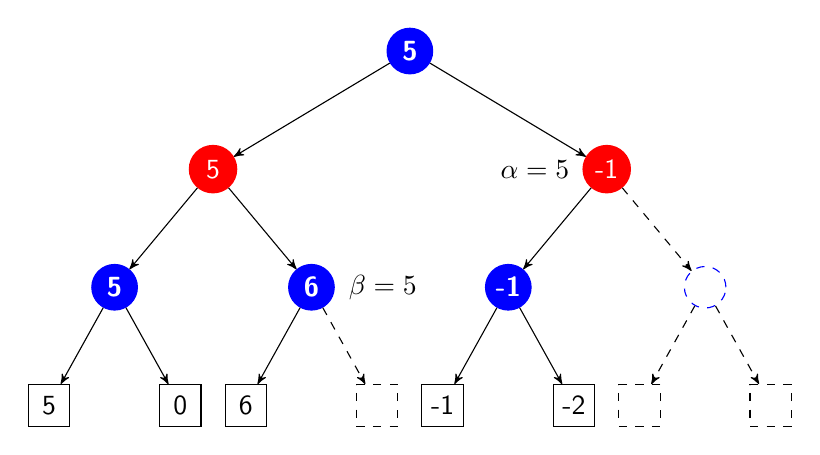
\begin{tikzpicture}[->,>=stealth',level/.style={sibling distance = 5cm/#1,
    level distance = 1.5cm}] 
\node [arn_n] {5}
child{ node [arn_r] {5} 
    child{ node [arn_n] {5}
        child{ node [arn_x] {5}}
        child{ node [arn_x] {0}} 
    }
    child{ node [arn_n] {6}
        child{ node [arn_x] {6}}
        child[dashed]{ node [arn_x] {}}
        node[right = 1em]{$\beta=5$}
    }                            
}
child{ node [arn_r] {-1}
    child{ node [arn_n] {-1} 
        child{ node [arn_x] {-1}}
        child{ node [arn_x] {-2}}
    }
    child[dashed]{ node [arn_n, fill=white] {}
        child{ node [arn_x] {}}
        child{ node [arn_x] {}}
    }
    node[left = 1em]{$\alpha=5$}
}
; 
\end{tikzpicture}
\end{center}

Die gestrichelten Teile sind nun (mögliche) Teilgraphen, welche mit dem normalen MiniMax Algorithmus hätten evaluiert werden müssen. In diesem Beispiel konnten wir uns 3/8 Blättern ignorieren können.

\section{Abgrenzung / Vergleich zu den vorherigen Kapitel}

In den vorherigen Kapiteln haben wir verschiedene Suchalgorithmen (Bestensuche, Branch-and-Bound, A*) kennengelernt. Diese liefern den Pfad, der zu dem Blatt mit dem höchsten Nutzwert führt. Jedoch beachten sie nicht, ob der Gegner auch diesen Pfad wählen würde. Der Gegner würde versuchen den geringsten Nutzwert für uns zu erreichen und somit versuchen von diesem Pfad abzuweichen. Folglich würden sie keine realistische Einschätzung darüber geben, welche Züge das beste Spielergebnis liefern. Im Gegensatz dazu betrachten sowohl der Minimax, als auch der Alpha-Beta Algorithmus das Verhalten des Gegners, welches zu einer guten Einschätzung der Spielsituation führt.



\section{Fazit \& Bewertung}

Zusammenfassend lässt sich sagen, dass der Minimax- und der Alpha-Beta-Algorithmus zum selben besten Ergebnis für den MAX-Spieler führen und sich lediglich in ihrer Effizienz unterscheiden können, da der Alpha-Beta-Algorithmus weniger Berechnungen und somit eine kürzere Rechnungszeit benötigen kann. Je nach Suchbaum kann die Anzahl der Cutoffs und die Einsparung der Rechenzeit sehr groß ausfallen. Aufgrund dessen ist der Alpa-Beta-Algorithmus eine Grundlage für viele Algorithmen im Bereich der Nullsummenspiele für zwei Personen. Für die Berechnungen der Algorithmen sind die Werte der Blätter von größer Bedeutung, welche durch die Heuristik gegeben sind. Alles in allem kann man sagen, dass man sowohl mit Minimax als auch mit Alpha Beta einen Computergegner programmieren kann, der es einem Menschen sehr schwer, wenn nicht sogar unmöglich, macht zu gewinnen und somit eine künstliche Intelligenz bei Nullsummenspielen für die Zukunft denkbar ist.


\section{Quellen und Literatur}

\begin{itemize}
\item MIT - Lecture 6: Search: Games, Minimax, and Alpha-Beta
\item http://home.in.tum.de/~adorf/pub/alphabeta-seminar-paper.pdf
\item https://de.wikipedia.org/wiki/Minimax-Algorithmus
\item https://de.wikipedia.org/wiki/Alpha-Beta-Suche
\end{itemize}
